\section{Design}
\label{sec:design}

\Syndicate\ defines a cloud storage abstraction, called a
{\it Volume}, that organizes application data across underlying storage.
An object written to a Volume is stored in its
cloud storage providers according to application storage policies, and
later delivered to readers via its edge cache providers.
Within a Volume, objects are organized into a filesystem-like directory
hierarchy, with an additional
control interface that lets administrators trade-off read
performance and data consistency.

\Syndicate's consistency protocol is central to 
implementing the Volume abstraction, since the protocol
covers its data, metadata, and control plane information.  We
describe the protocol in two phases.
First, we assume that the relevant components have 
fresh metadata, and show how they use it to overcome weak cache consistency
without losing the benefits edge caches offer.  Second, we show how 
they obtain fresh metadata in a scalable manner.  We then
show how \Syndicate\ implements fault tolerance,
storage layer security, and storage policies, using the
consistency protocol to distribute the necessary control plane information.

\subsection{Components}

\Syndicate\ consists of two components: a set of peer {\it \Syndicate\
  Gateways} (\SG), and a scalable {\it Metadata Service} (\MS).  \SGs\
are the middleware processes that interface between \Syndicate\ and
the existing storage elements, and work together to implement the
Volume abstraction for applications by managing object data.
The \SGs\ coordinate to meet consistency, security, and 
storage policies via a shared \MS, 
which itself manages object metadata and facilitates Volume administration.

The \SG\ comes in three variants, depending on how it interfaces with
the outside world:

\begin{description}

\item[\bf User \SG:] Interfaces with user/application processes in
  order to implement the Volume abstraction.  Responds to both locally
  generated read/write requests and read/write requests from peer \SGs.  Our
  prototype offers three application-facing interfaces: a
  FUSE~\cite{fuse} filesystem, a RESTful Web
  object store, and a Hadoop Filesystem~\cite{hdfs} front-end.

\item[\bf Replica \SG:] Uploads written data to cloud storage
  providers on behalf of the Volume, and later downloads it and serves
  it to edge caches on demand.  Responds to read/write requests from peer
  \SGs, but does not generate any local requests. Our prototype
  currently supports Amazon S3~\cite{aws-overview}, Dropbox~\cite{dropbox},
  Box.net~\cite{Box.net}, Google Drive~\cite{google-drive}, Amazon
  Glacier~\cite{aws-overview}, and local disk as back-end storage.

\item[\bf Acquisition \SG:] Maps existing data sets
  into one or more Volumes as a read-only directory hierarchy.
  Responds to read (but not write) requests from peer \SGs, but does not
  generate any local requests. Our prototype currently supports
  GenBank~\cite{GenBank}, Common Crawl~\cite{common-crawl}, and M-Lab~\cite{mlab} data sets.

\end{description}

\noindent Although there are three variants of the \SG, they all play
the same role in the larger \Syndicate\ design, and so we do not
distinguish among them unless critical to understanding the system.

\begin{figure}[h!]
\centering
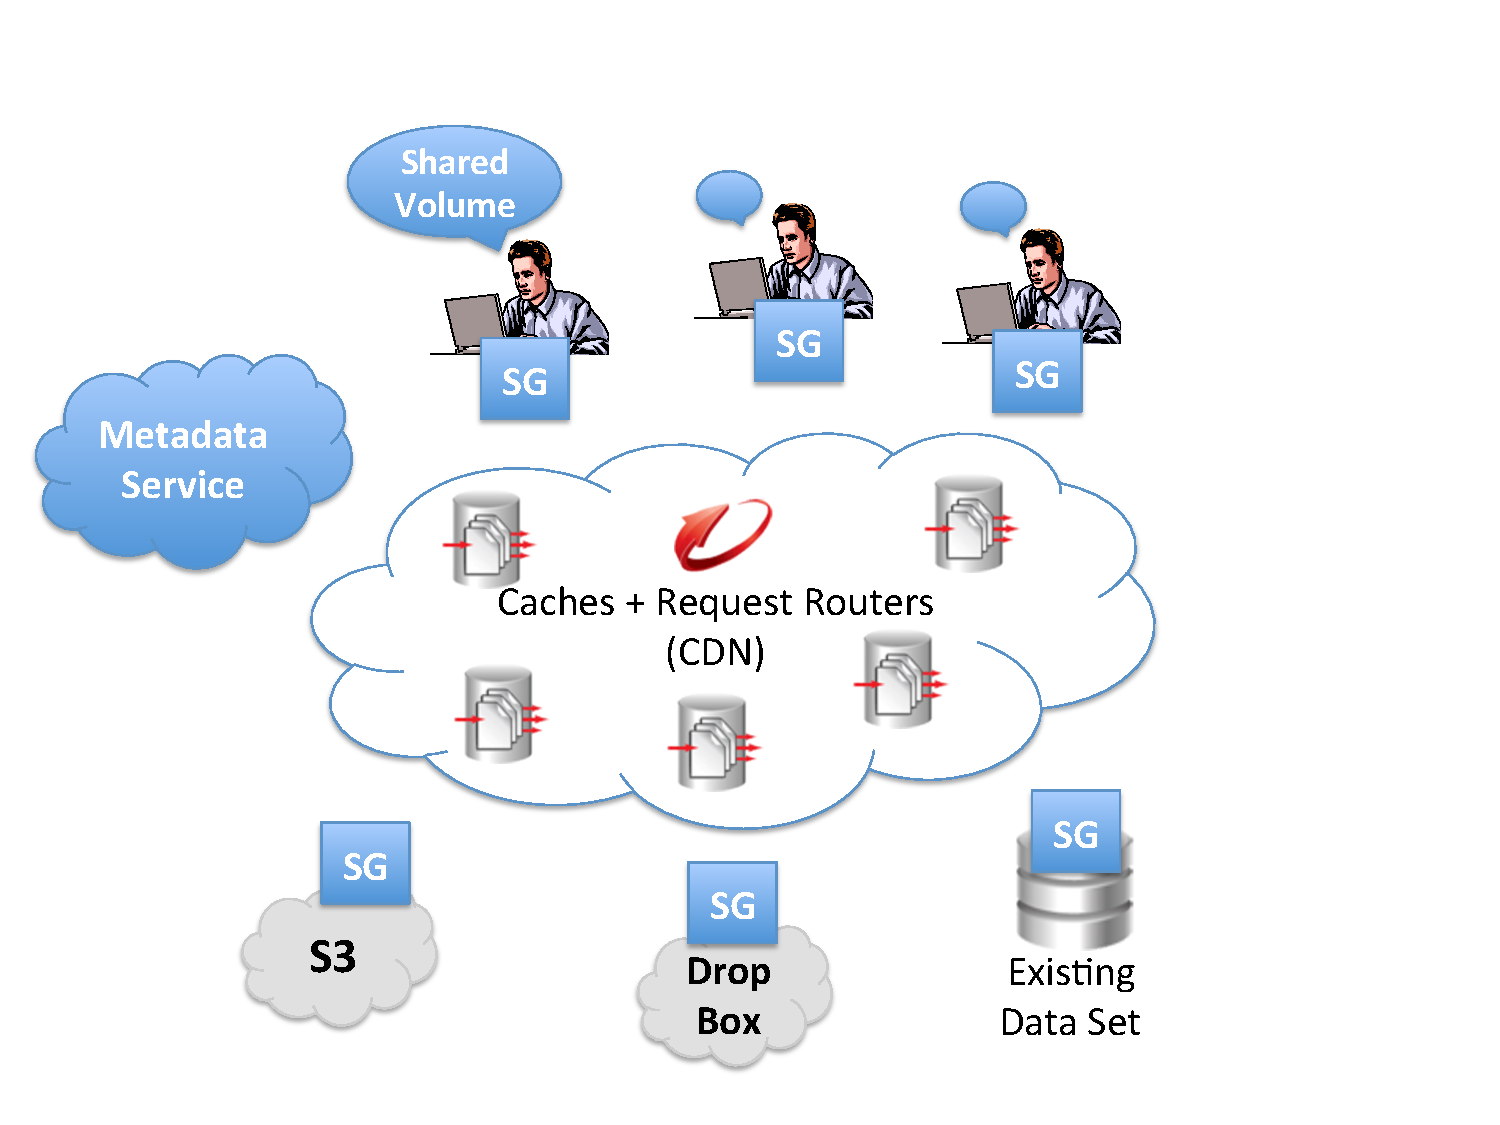
\includegraphics[width=0.5\textwidth]{figures/Syndicate-fig}
\caption{\it Example deployment of \SGs\ between edge caches, cloud storage, existing data sets, and application local storage.}
\label{fig:deployment}
\end{figure}

In a typical deployment (Figure~\ref{fig:deployment}), an application 
has one \MS, and places its objects into one or more Volumes.
Each host runs an \SG\ locally for each Volume to which
it has access, so processes only see the intended data.
The application developer deploys additional \SG\ instances to
allow the application to store and later retrieve data from cloud
storage, and to optionally read (but not write to) external existing 
data sets.

\subsection{Object Data and Consistency}

To manage a scalable number of objects, \Syndicate\ divides
responsibility for them among the
\SGs\ in the Volume.  Each object in \Syndicate\ is assigned
one \SG\ to act as its coordinator.  A coordinator
has two responsibilities:  implementing data plane
consistency with the help of the \MS, and processing writes
from other \SGs.

It is difficult to download fresh data from HTTP-speaking
edge caches because they do not always honor cache control directives,
for example, due to bugs, misconfiguration, or intentional shunning by
the edge cache operator.  Thus to obtain fresh data, \SGs\ use HTTP
URIs that uniquely identify the latest snapshot of the data, obviating
the need for them.  The challenges are to use cache capacity efficiently,
and ensure \SGs\ discover the correct URIs before downloading.

To address the former, \SGs\ serve object data as fixed-sized blocks
(the size is application-defined).
To address the latter, a coordinator \SG\ stores two records for each block:  
a block nonce that uniquely identifies its current contents, and the set of which \SG(s)
can serve a copy.  It additionally stores a unique object
generation nonce assigned on creation, and a monotonically-increasing object
last-write timestamp.  It keeps track of this information using an object
\textit{manifest} (Figure~\ref{fig:manifest}), and uses this information
to generate block URIs.

\begin{figure}[h!]
\centering
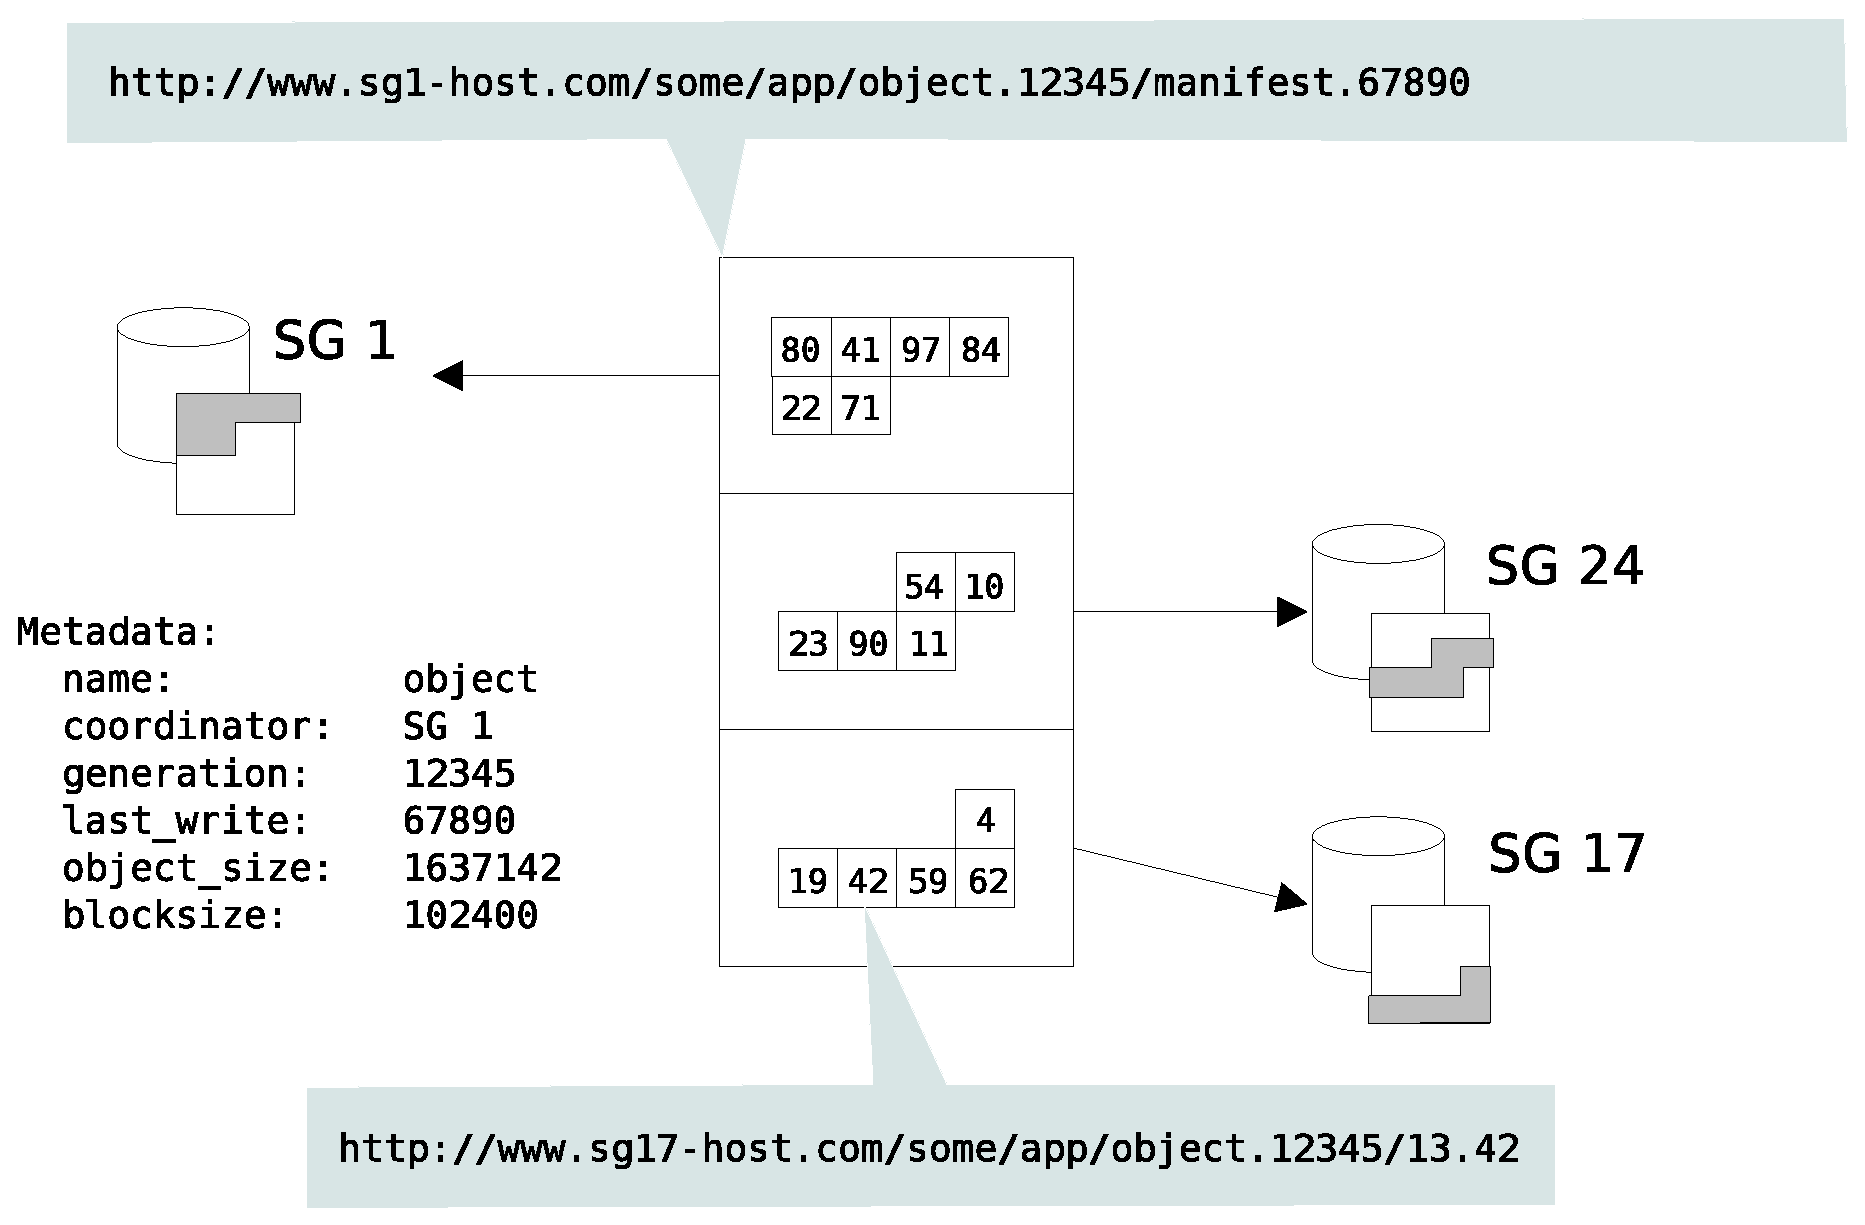
\includegraphics[width=0.5\textwidth]{figures/manifest}
\caption{\it Logical representation of a manifest for a 16-block object after 
three writes.  Each \SG\ (cylinders) hosts the latest 
copies of some of the object blocks (grey areas), which the manifest tracks.  Generation nonces,
last-write timestamps, and block nonces are kept short for brevity.}
\label{fig:manifest}
\end{figure}

To read an object, an \SG\ first obtains the object's latest generation nonce 
and last-write timestamp from the \MS.  Then, it generates an HTTP URI for the manifest using 
these two records, as well as the object's path.  By including these records,
the URI to the manifest will identify a snapshot as fresh as the records indicate.
This allows the \SG\ to download the manifest from the coordinator via the edge caches
and receive fresh data.

Once obtained, the manifest lets the reader construct 
URIs for each of the object's blocks.  A block URI
includes the path to the object in the Volume, the generation nonce,
the block ID, and the block nonce.  Because the block nonce 
changes whenever the block is modified, the URI will change whenever the block 
changes.  This way, the \SG\ can distribute data with unmodified 
edge caches and guarantee that readers see data as fresh as the manifests indicate.

When an \SG\ writes to an object, it first obtains fresh metadata and 
manifest data, and sends the modified blocks
to a Replica \SG\ in the Volume for archival to cloud storage.  The writer then generates 
new nonces for the modified blocks and sends them
to the coordinator.  Upon receipt, the coordinator generates a new last-write
timestamp, adds the block nonces in the manifest, and uploads the manifest to 
a Replica \SG\ as well.  It then sends the last-write timestamp
to the \MS\ for subsequent readers to fetch.
It finally acknowledges the writer \SG, completing the write operation.

% TODO: would a figure showing a read and write execution trace be helpful? -jcn

From a consistency standpoint, \Syndicate\ 
ensures readers receive data as up-to-date as the downloaded manifest,
which itself is as up-to-date as the object metadata from the \MS.
By default, the \SG\ offers last-write-wins semantics, which is adequate for our sample
applications, and is comparable to what 
cloud storage providers offer today (although other semantics are possible).
Reads and writes are not atomic with respect to one another, but
synchronously fetching new metadata and manifests on each read
yields per-object sequential consistency, with writes observed in the
coordinator-observed order.  By varying how stale cached metadata 
and manifests are allowed to become, the \SG\ can trade stronger 
consistency for faster access (Section~\ref{sec:metadata-consistency}).

The \SGs\ cache manifests and
block data for locally-read objects, and continue to host
recently-written data 
after it has been backed up.
Once durable, hosted data is
evicted once they become remotely  
overwritten, or if they are infrequently
accessed.  Manifests for the objects 
the \SG\ coordinates are always kept resident.
We allow an application to 
control this policy per-object, in order
to guarantee that the object's data 
remains locally available for fast and/or off-line access.

\subsection{Metadata and Consistency}
\label{sec:metadata-consistency}

While \SGs\ handle reads and writes on object data, the \MS\ helps
them coordinate to implement data consistency.  Specifically, \SGs\ rely on the \MS\ to
announce their presence, to announce the objects they coordinate,
to discover other \SGs\ and their objects, and to help them read sufficiently
recent object data from one another.

The \MS\ maintains a metadata record for every object and directory in 
each Volume, as well as records for each \SG.
An object/directory record is functionally similar to an i-node,
except that it does not track blocks (this is handled by the 
object manifest).  A listing of relevant fields the 
\MS\ tracks can be found in Table~\ref{tab:metadata}.

\begin{table}[ht!]
\begin{tabular}{ | l | l |}
\hline
\textbf{Name} & \textbf{Description} \\
\hline
\texttt{type} & Object or Directory record.\\
\texttt{name} & App-chosen record name. \\
\texttt{object\_id} & Volume-wide unique object ID. \\
\texttt{user\_id}  & App user ID that owns this object. \\
\texttt{coord\_id} & ID of the coordinator \SG. \\
\texttt{volume\_id} & Which Volume contains this object.\\
\texttt{generation} & Object generation nonce. \\
\texttt{last\_write} & Object last-write timestamp. \\
\texttt{perms} & Permissions for this object. \\
\texttt{read\_ttl} & Cached lifetime on an \SG. \\
\hline
\end{tabular}
\caption{\it Partial list of fields kept in each record by the Metadata Service.}
\label{tab:metadata}
\end{table}

The \MS\ serves as the coordinator for all directories in a Volume, 
and processes object/directory creation and deletion requests on behalf of the 
Volume's \SGs.  As such, creations and deletions
within a given directory are serialized, ensuring that a directory's
immediate children have unique names.  This ensures that an object 
URI refers to at most on object, as desired.

The freshness of an object's data is determined by how fresh the 
object's cached metadata is on the \SG, which applications
control to trade consistency (freshness) for read performance
To do so, \Syndicate\ gives each object and directory an
application-set {\tt read\_ttl} field that
tells the \SG\ for how long metadata can be assumed fresh after it is downloaded.
This is functionally equivalent to applying cache-control directives used today,
and provides delta consistency~\cite{delta-consistency} when {\tt read\_ttl} is non-zero
(a value of zero provides sequential consistency).
\Syndicate\ additionally lets an application invalidate cached metadata,
if it needs the next read operation to obtain fresh data.

{\bf Metadata Consistency Protocol.}  Since \Syndicate\ is intended for
read-heavy workloads, we assume
that directories are rarely added or removed relative to the
how often they or their children are accessed.  For this reason,
\SGs\ locally cache and revalidate metadata grouped by 
directory listings, and only redownload listing when they discover that 
it has changed on the \MS.  This way, most of the time, the \SG\ will 
have a locally cached (but potentially stale) listing for each directory
along the paths to the objects it accesses.

When given a path to an object, the \SG\ 
first walks down the cached directory listings along the path.
It breaks the path into three disjoint segments 
of directory listings:  the longest prefix along the path where each listing is both
cached and fresh ($P_{fresh}$), the segment of listings after this prefix that starts
with a locally cached but stale listing ($P_{stale}$), and the segment of
listings after $P_{stale}$ that are not locally cached ($P_{absent}$).

% TODO: should we add a figure of the above, to drive the consistency protocol home?
% -jcn

The \SG\ does not need to revalidate the listings in $P_{fresh}$, but will need to revalidate 
every listing in $P_{stale}$ since
undiscovered changes in them can affect all subsequent listings.  To do so,
the \SG\ sends the \MS\ the cached {\tt object\_id} and {\tt last\_write} fields of each
listing's directory.  For each directory given, the \MS\ will return the new listing if it has 
a different {\tt last\_write} value than indicated by the \SG. 
Otherwise, it either responds with a
``Not Modified'' message if the directory has the same last-write timestamp,
or with a ``Not Found'' message if the directory does not exist or the \SG\
is no longer allowed to search it.

After processing the \MS\ response, every directory listing in $P_{stale}$
will be fresh.  Then, for each listing in $P_{absent}$, the \SG\ sequentially downloads
and caches each listing in order to learn the {\tt object\_id} for the next listing (which 
is necessary to request it).  Once all listings in $P_{absent}$ have 
been downloaded, every listing along the path will be fresh,
and the \SG\ can proceed to access the object (whose fresh metadata is contained
in its parent directory's listing).

The intuition behind this protocol is that it usually costs at most
one RTT when objects exhibit access locality.
When an object is accessed multiple times,
directories that had been in $P_{absent}$ the first time will likely 
be in either $P_{fresh}$ or $P_{stale}$ afterwards, meaning
$P_{absent}$ is usually empty.  So, the cost of obtaining fresh 
object metadata, fresh path metadata, and checking search permissions
is usually the cost of revalidating $P_{stale}$.  The \SG\ will
not need to contact the \MS\ at all if
$P_{fresh}$ includes the entire path, or 
if $P_{stale}$ is empty and $P_{absent}$ is not (in which case, the 
object can be inferred not to exist).

\subsection{Provider Composition}
\label{sec:composition}

% TODO: avoid gratuitous formalisms?
% -jcn

Beyond consistency, applications have domain-specific,
changing storage policies.
To meet them, \Syndicate\ automatically and securely
distributes developer-supplied idempotent closures to \SGs,
which \SGs\ call on reads and writes.
They are used for achieving compatibility with specific 
providers, and enforcing storage policies.

When a user provisions an \SG, she supplies the \MS\ a read-only configuration
$C$, a read function $R$, and a write 
function $W$.  When it receives a read request for a manifest or block, the
\SG\ will run $R$ with $C$ to obtain the requested data.
When it receives a write with new manifest or 
block data, it will run $W$ with $C$ to process it.

The functional differences between \SGs\ lie mostly in how they implement $R$
and $W$.  For a User \SG, $W$ writes block data to local storage
using last-write-wins write conflict resolution.
$R$ translates a read request and the object metadata
into cache-specific HTTP GET requests, and downloads 
the data from them.

The Replica \SG\ uses $W$ and $C$ to upload manifest and block data
to underlying providers, and uses $R$ and $C$ to retrieve them later.
It ensures $W$ is idempotent and space-efficient by uploading a data record
unique to the version of the data, and garbage-collecting stale data.
An Acquisition \SG\ has no $W$, but uses $R$ to match an object path 
to a per-object function $R_{object}$.  $R_{object}$ will be run 
to generate the requested data from the underlying data set and perform internal caching.

Using closures in this way decouples the storage policies from the provider,
creating a marketplace of reusable $R$ and $W$ implementations.
Compatibility with a provider only needs to be addressed once for many applications,
and enforcement of higher-level policies, such as data compression, encryption,
erasure coding, logging, and so on, can be embedded into these closures.
Additionally, per-application optimizations such as write-batching 
or asynchronous replication can be addressed with them.

$C$, $R$, and $W$ may be modified
on a live system---for example, to update credentials, distribute keys, or fix bugs.
To address this, \Syndicate\ treats them as special data objects. \SGs\ will
periodically refresh closure metadata and re-download new copies automatically,
using the edge caches to scale read bandwidth.

In practice, $C$ contains sensitive information, such as account credentials
or encryption keys.  To securely distribute $C$, the developer first 
obtains the \SGs' public keys and encrypts each \SG-specific record
with the appropriate key.  She then signs $C$, $R$, and $W$ before uploading them.
In this capacity, as long as the user can securely obtain the \SG's public keys,
she can rely on \Syndicate\ to securely distribute her closures in a scalable manner.  We address this in more detail in Section~\ref{sec:security}.

\subsection{Scalability and Fault Tolerance}
\label{sec:controlplane}

Our scalability and fault tolerance goals for \Syndicate\ are to ensure that 
it is not a performance bottleneck for an application, and that 
it is available to process reads and writes despite \SG\ failures.
To achieve this, \Syndicate\ scales up and distributes Replica
\SG\ instances to meet write load, and automatically transfers object coordinator
responsibilities between \SGs\ when they fail.

\Syndicate\ cannot make progress if the \MS\ is offline.
To address this, we designed the \MS\ to be portable across 
many cloud computing platforms and compatible with many highly-available 
NoSQL store implementations, allowing the developer to choose a sufficiently
reliable cloud computing platform.

To scale application writes, \Syndicate\ instantiates and runs Replica
\SGs\ across an application-chosen set of hosts, and distributes requests
to them with an existing HTTP/DNS load balancer with failure detection.
Because $R$ and $W$ are idempotent, a read or write on a failed Replica \SG\ instance
is simply restarted.

By default, an object's coordinator is simply the \SG\ that created it.
If the coordinator fails or becomes unavailable, a reader 
\SG\ will simply fetch the object manifest and blocks from a Replica \SG.  A 
writer \SG\ will attempt to become its new coordinator, so it can process 
its write (and subsequent writes).  Note that although Replica \SGs\ receive
written object data, they are forbidden from serving as coordinators for security reasons.

If a coordinator \SG\ is unresponsive to a writer, the writer
requests the \MS\ to set the object's {\tt coordinator} field to itself.
If the \MS\ approves, the \SG\ reads the latest copy of its manifest from a Replica \SG, updates
it to list the Replica \SG\ as the host for all of the blocks,
and then performs its write as normal.  The other \SGs, including the original
coordinator, will detect the change when they next refresh its metadata.
A read sent to the wrong coordinator \SG\ will either be redirected (on cache miss)
or will be served ``stale'' data that is less stale than the object's {\tt read\_ttl} allows
(on cache hit).

If multiple \SGs\ attempt to become the new coordinator, the \MS\
picks the first \SG\ as the winner, increments the object's last-write timestamp,
and tells the remaining \SGs\ to instead
refresh the object's metadata and restart their writes.  This means
if a set of writer \SGs\ are partitioned from one another, they will ``take turns''
becoming the coordinator as needed until they re-establish contact.
Depending on application needs, intermittent writes will either fail fast (i.e. the 
application is instructed to try again) or be restarted internally if 
the wrong coordinator attempts to process them.

Any User \SG\ with the right capabilities can become the coordinator of an
object in the Volume, provided the object has the appropriate permission  
set in its {\tt perms} field.  The application can also explicitly 
move an object between allowed coordinators.
This is because the application ``knows best'' how to  
to place its objects across \SGs---for example, a VDI application
would try to coordinate VM images with \SGs\ close
to its user, but an online document editor would try to distribute
documents across its servers' \SGs\ to balance load.

\subsection{Security}
\label{sec:security}

To address security, \Syndicate\ concerns itself with providing
a trusted storage layer on top of an application's hosts,
using the application to bootstrap trust between components.  This 
lets the application developer avoid trusting existing services,
and creates an environment for the application to securely implement 
data privacy and distribute sensitive control-plane information.

Our threat model assumes that eavesdroppers (Eve) can read data on the network, but not 
within \Syndicate\ components or the \MS's storage.  We also assume that malicious 
agents (Mal) try to spoof the \MS\ and \SGs, and try to compromise \SGs.
As such, \Syndicate\ ensures that only authorized \SGs\ may participate
in a Volume, and only if they are running on behalf of their user on
a designated host/port.  Even then, they may only interact with
the Volume according to developer-given capabilities.

To enforce this, each Volume acts as a certificate authority for
its \SGs.  The Volume maintains a signed certificate for each of its \SGs, identifying
the information listed in Table~\ref{tab:sg-cert}.  Each \SG\ 
keeps a certificate bundle for all other \SGs\ in the same Volume.

\begin{table}[ht!]
\begin{tabular}{ | l | p{5cm} |}
\hline
\textbf{Field} & \textbf{Description} \\
\hline
\texttt{pubkey} & The \SG's current public key.\\
\texttt{hostname} & The host on which the \SG\ runs. \\
\texttt{port} & The port on which the \SG\ listens. \\
\texttt{user\_id}  & App user ID running the \SG. \\
\texttt{volume\_ids} & IDs of this \SG's Volumes.  \\
\texttt{capabilities} & The \SG's per-Volume capabilities. \\
\texttt{issued} & Certificate issue date. \\
\texttt{expires} & Certificate expiration date. \\
\texttt{revoked} & Revocation status of this certificate. \\
\hline
\end{tabular}
\caption{\it Summary of the fields kept in an \SG\ certificate.}
\label{tab:sg-cert}
\end{table}


To distribute and revoke certificates at scale,
\SGs\ treat their certificate bundle as a \Syndicate\ object,
where each certificate is a block.
The \MS\ and \SGs\ gossip its cryptographic hash and last-write timestamp.
When either value changes (due to the addition or revocation
of a certificate), the \SGs\ synchronize their certificate bundle with the \MS\ by
fetching the bundle's manifest, fetching new certificate data through edge caches,
and deleting \MS-revoked or expired certificates.

The application bootstraps trust between the \SG\ and the \MS.
When the developer installs an \SG\ on a host, she gives it a set of secret 
credentials to use to register itself with the \MS\ upon instantiation.  It
submits these credentials (via TLS) to an OpenID~\cite{openid} provider,
which the \MS\ is configured to trust
(i.e. either a 3rd party one, or one built into the application logic).
It then vouches for the authenticity of both components to each other.

Once authenticated, the \SG\ generates a public/private key pair for this
session (or uses one given by the application), sends the \MS\ the public key,
and receives the Volume's public key and root directory listing.
The \MS\ then generates and distributes a new certificate
for it.  The \SG\ will periodically renew its certificate, but the \MS\ will revoke it
if it expires, if the \SG\ shuts down normally, or if the developer stops trusting it.

With the exception of data served to the edge caches, \Syndicate\ uses TLS to 
secure all messages between its components.  Each message is signed by
the sender, allowing other components to ignore unverifiable messages.  This
scheme prevents Eve from reading control-plane data, and prevents Mal from spoofing components.

A compromised \SG\ is limited to damaging its Volume(s), and only as far as 
its capabilities allow.  These capabilities are used to ensure that an Acquisition \SG\
is only allowed to create a limited number of read-only objects and directories
(the \MS\ takes care of deleting them when its certificate is revoked).
They also ensure that a Replica \SG\ may never interact with Volume metadata
beyond pulling new certificate data.

To limit the damage Mal can do with a compromised User \SG, an application can
specify for an entire Volume which \SGs\ have the capability
to write to objects, and which can coordinate objects (without either,
a User \SG\ is read-only, and does not participate in certificate distribution).
In addition, the application compartmentalizes data by partitioning objects across 
multiple Volumes.

%\subsection{Discussion}
%\label{sec:discussion}

%TODO---do we even need anything here?